\subsection{Trådløs kommunikation}\label{traadloes_komm_imp}
Den trådløse kommunikation er tiltænkt direkte kommunikation mellem mikrokontrolleren og prototypen, hvorved exoskelettet kan styres. 
Herudover skal der etableres en trådløs forbindelse til en computer til debugging og test af mikrokontrolleren samt datavisualisering.   

\noindent
Til implementeringen af den trådløse kommunikation tages der ikke udgangspunkt i det oprindelige design, som er beskrevet i \autoref{sec:traadloes_komm_design}. 
Dette er grundet, at opsætningen af BLE-kommunikationen i mikrokontrolleren er mere kompliceret end først antaget.
Af denne grund vælges det at implementere et mere simpelt og anvendeligt alternativ, bestående af to PSoC 4 M-Series Prototyping Kit boards, der ses af \autoref{fig:PSoC_4200}. 
Disse vil efterfølgende refereres til som 'gumsticks'. 

\begin{figure}[H]
	\centering
	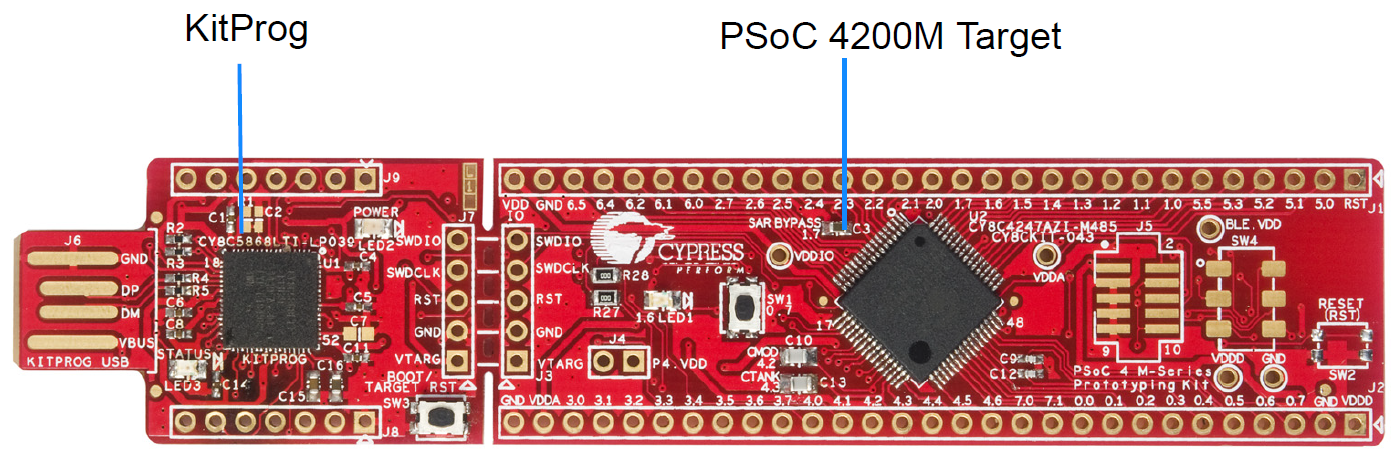
\includegraphics[width=0.8\textwidth]{figures/PSoC_4200_opdelt}
	\caption{Opbygningen af en gumstick. Denne komponent består af en KitProg og en PSoC 4200M target \citep{cypresspsoc42015}.}
	\label{fig:PSoC_4200}
\end{figure}

\noindent
Gumstickens board på \autoref{fig:PSoC_4200} består af en KitProg og en PSoC 4200M enhed. KitProgen anvendes til at debugge og programmere koden. PSoC 4200M er enheden, hvorpå processoren er placeret og hvor koden eksekveres. 
Yderligere er boardet udstyret med et EZ-BLE modul, der tillader trådløs kommunikation ved brug af BLE. Dette modul er tilsluttet på bagsiden af gumsticken, og fremgår dermed ikke af \autoref{fig:PSoC_4200}. 

Den ene gumstick tilkobles mikrokontrolleren via en Universal Asynchronous Receiver/Transmitter (UART)-forbindelse, der både kan sende og modtage data ved at forbinde mikrokontrollerens transmitter (TX) med gumstickens receiver (RX) og forbinde mikrokontrollerens RX med gumstickens TX. 

Den anden gumstick tilsluttes computeren via en USB-forbindelse og erstatter BLE-donglen fra det oprindelige design. En illustration af, hvordan kommunikationen transmiteres i det implementerede system fremgår af \autoref{fig:Traadloes_Komm_Imp}.

\begin{figure}[H]
	\centering
	\includegraphics[width=0.8\textwidth]{figures/traadloes_komm}
	\caption{Illustration af kommunikation mellem mikrokontroller og computer. Der ses UART-forbindelse til venstre, hvor RX og TX er forbundet mellem mikrokontrolleren og den centrale gumstick. Til højre ses indikeringen af trådløs kommunikation ved brug af BLE \citep{cypresspsoc2015, cypresspsoc42015}.} 
	\label{fig:Traadloes_Komm_Imp}
\end{figure}

\noindent
Opsætningen, der fremgår af \autoref{fig:Traadloes_Komm_Imp}, er mere anvendelig, da der findes kodeeksempler til gumsticken, hvorpå den trådløse kommunikation er programmeret. 
Dertil er det ikke nødvendigt at opsætte BLE-kommunikation, men kun hvordan dataen skal videregives. 
Begge gumsticks programmeres til at gengive information, der modtages via BLE eller UART. 
Dertil vil data modtaget fra mikrokontrolleren blive videregivet til den ene gumstick, hvorpå data transmiteres trådløst til den anden gumstick. 
Derfra sendes data via UART til computeren. 

For at de to gumsticks kan kommunikere med hinanden, progammeres EZ-BLE modulerne til at være henholdsvis central og perifer. 
Dette betegner en rolle, der gives til de to gumsticks. 
Central er oftest enheden med mest processorkraft og hukommelse, og den perifere er oftest enheden med mindre processorkraft og som er ressourcebegrænset \citep{townsend2014}. 
I dette system er central og perifer opsat som illustreret på \autoref{fig:Traadloes_Komm_Imp}. 
Mikrokontrolleren bliver anset som en primær komponent, hvortil den UART-forbundne gumstick defineres som central. 
Gumsticken, der modtager data via BLE, bliver dermed perifer. 
Ved aktiv datatransmission vil dette indikeres ved en blå LED.